\documentclass[10pt,twocolumn,letterpaper]{article}

% Barang-barang saya sendiri
\usepackage{booktabs}
% \usepackage{caption}
% \captionsetup[table]{skip=8pt}   % Hanya mempengaruhi tabel
\usepackage{stfloats}  % Tambahkan ini ke preamble
\usepackage{float}

\usepackage{cvpr}
\usepackage{times}
\usepackage{epsfig}
\usepackage{graphicx}
\usepackage{amsmath}
\usepackage{amssymb}

% Sertakan paket lain di sini, sebelum hyperref.

% Jika Anda mengomentari hyperref lalu membatalkannya, Anda harus menghapus
% egpaper.aux sebelum menjalankan latex lagi.  (Atau cukup tekan 'q' pada latex pertama
% run, let it finish, and you should be clear).
\usepackage[breaklinks=true,bookmarks=false]{hyperref}

\cvprfinalcopy % *** Uncomment this line for the final submission

\def\cvprPaperID{****} % *** Enter the CVPR Paper ID here
\def\httilde{\mbox{\tt\raisebox{-.5ex}{\symbol{126}}}}

\renewcommand{\tablename}{Tabel}
\renewcommand{\figurename}{Gambar}   % or whatever you like instead of "Hình"
\renewcommand{\refname}{Referensi}

\makeatletter
\def\abstract{%
  \centerline{\large\bf Abstrak}% <-- your new label
  \vspace*{12pt}%
  \it%
}
\makeatother

% Pages are numbered in submission mode, and unnumbered in camera-ready
%\ifcvprfinal\pagestyle{empty}\fi
\setcounter{page}{1}
\begin{document}

%%%%%%%%% TITLE
\title{Pengantar ECDO Berbasis Data Bagian 1/2: Pemahaman Terkini tentang Teori “Pembalikan Bumi” Osilasi Dzhanibekov Pelepasan Inti-Mantel Eksotermik (ECDO)}

\author{Junho\\
Diterbitkan Februari 2025\\
Website (Unduh makalah di sini): \href{https://sovrynn.github.io}{sovrynn.github.io}\\
Repositori Riset ECDO: \href{https://github.com/sovrynn/ecdo}{github.com/sovrynn/ecdo}\\
{\tt\small junhobtc@proton.me}
% Untuk makalah yang semua penulisnya berasal dari institusi yang sama,
% abaikan baris-baris berikut hingga penutup ``}''.
% Penulis dan alamat tambahan dapat ditambahkan dengan ``\and'',
% seperti penulis kedua.
% Untuk menghemat ruang, gunakan alamat email atau halaman rumah, jangan keduanya
% \and
% xxx
% Institusi2\\
% Baris pertama alamat institusi2\\
% {\tt\small secondauthor@i2.org}
}

\maketitle
%\thispagestyle{empty}

%%%%%%%%% ABSTRACT
\begin{abstract}
Pada bulan Mei 2024, seorang penulis daring dengan nama samaran “The Ethical Skeptic” \cite{0} memposting sebuah teori terobosan yang disebut Osilasi Dzhanibekov Pelepasan Inti-Mantel Eksotermik (ECDO: Exothermic Core-Mantle Decoupling Dzhanibekov Oscillation) \cite{1}. Teori ini tidak hanya mengemukakan bahwa Bumi sebelumnya pernah mengalami pergeseran mendadak dan katastropik pada sumbu rotasinya—yang menyebabkan banjir besar global akibat lautan tumpah ke daratan karena inersia rotasi, tetapi juga menyajikan mekanisme geofisika yang mendasarinya, berdasarkan data empiris yang mengindikasikan bahwa peristiwa serupa berpotensi terjadi kembali dalam waktu dekat. Walaupun ramalan tentang banjir katastropik dan kiamat bukanlah hal baru, teori ECDO sangat menarik karena pendekatannya yang ilmiah, modern, multidisipliner, dan berbasis data.

Makalah penelitian ini merupakan bagian pertama dari rangkuman singkat dua bagian atas enam bulan penelitian independen \cite{2,20} tentang teori ECDO. Makalah ini menyoroti tiga poin utama:

\begin{flushleft}
\begin{enumerate}
    \item Peristiwa 'pembalikan Bumi' yang menyerupai ECDO telah terjadi beberapa kali dalam sejarah manusia baru-baru ini, sebagaimana dibuktikan oleh berbagai mitos banjir besar serta jejak-jejak geologis banjir yang pernah menutupi wilayah benua
    \item Arah dan besaran pembalikan Bumi di masa lalu dapat diestimasi dengan cukup akurat.
    \item Data geomagnetik dan geofisika terbaru mengindikasikan bahwa pembalikan Bumi berikutnya dapat segera terjadi, dan bahwa perubahan iklim mungkin disebabkan oleh perubahan yang terjadi di dalam inti Bumi, bukan oleh manusia.
\end{enumerate}
\end{flushleft}

Selain itu, saya membahas mekanisme fisika penyebab di balik fenomena “pembalikan Bumi” yang diajukan oleh teori ECDO.

Dalam makalah ini, saya tetap bersikap objektif dengan berfokus pada data empiris, menghindari bagian-bagian teori yang menarik namun masih bersifat spekulatif, dan menekankan bahwa ini adalah topik yang sangat mendesak untuk diteliti lebih lanjut oleh umat manusia.
\end{abstract}

%%%%%%%%% BODY TEXT
\section{Pendahuluan}

Kisah tentang banjir besar bukanlah hal baru—faktanya, cerita-cerita seperti ini ditemukan pada setiap kebudayaan besar di seluruh dunia, di semua pusat peradaban. Pemetaan pada (Gambar \ref{fig:1}) adalah kompilasi dari 267 kisah banjir besar \cite{3}, yang menunjukkan bahwa hampir semua wilayah yang pernah dihuni oleh manusia di Bumi mempunyai cerita tentang banjir besar.

% \begin{figure}[h]
% \begin{figure}[b]
\begin{figure}[h]
\begin{center}
% \fbox{\rule{0pt}{2in} \rule{0.9\linewidth}{0pt}}
   \includegraphics[width=1\linewidth]{b.png}
\end{center}
   \caption{Daerah yang memiliki kisah banjir di seluruh dunia \cite{3}.}
\label{fig:1}
\label{fig:onecol}
\end{figure}

Jika kisah-kisah banjir ini ditelaah dengan lebih dekat, tampak jelas bahwa kejadian-kejadian tersebut bukanlah banjir biasa, melainkan bencana kataklismik yang bersifat destruktif disertai banjir dahsyat yang menyapu bersih seluruh benua.

\subsection{Cerita Bencana Suku Asli Amerika}

Cerita dari suku asli Amerika memuat beberapa kisah yang paling eksplisit tentang peristiwa kataklismik besar yang pernah terjadi di Bumi. Suku Hopi, salah satu suku asli Amerika yang tinggal di wilayah timur laut Arizona, mengatakan bahwa, \textit{"..Sótuknang memanggil Bangsa Semut untuk membuka dunia bawah tanah mereka bagi orang-orang terpilih. Ketika mereka telah berada di bawah tanah dengan aman, Sótuknang memerintahkan si kembar, Pöqánghoya dan Palöngawhoya, untuk meninggalkan pos mereka di ujung utara dan selatan sumbu dunia, tempat mereka ditempatkan untuk menjaga rotasi bumi supaya tetap stabil. \textbf{Baru saja si kembar itu meninggalkan pos mereka, dunia—tanpa ada yang mengendalikan—mulai kehilangan keseimbangan, berputar kacau, lalu terguling dua kali.} Gunung-gunung jatuh ke laut dengan hentakan besar, lautan dan danau meluap ke daratan; dan saat dunia berputar melewati ruang yang dingin dan tak bernyawa, dunia ini membeku menjadi bongkahan es padat"} \cite{4}.

Banyak dari cerita-cerita ini secara spesifik menggambarkan besarnya skala banjir besar yang terjadi, dengan menceritakan bagaimana lautan naik hingga menenggelamkan hampir semua daratan kecuali puncak-puncak gunung tertinggi. Suku Indian Skokomish, yang tinggal di negara bagian Washington, menceritakan bahwa, \textit{"Roh Agung, yang murka terhadap kejahatan manusia dan hewan, memutuskan untuk membersihkan bumi dari semua makhluk kecuali hewan-hewan baik, seorang pria yang baik, dan keluarganya. Atas petunjuk Roh Agung, pria itu menembakkan anak panah ke awan, lalu anak panah berikutnya ke anak panah pertama, dan seterusnya, hingga membentuk tali anak panah dari awan ke tanah. Hewan-hewan dan manusia yang baik memanjat naik. Hewan-hewan jahat dan ular mencoba ikut naik, tetapi pria itu memutuskan tali tersebut. \textbf{Kemudian Roh Agung menyebabkan hujan turun selama berhari-hari, membanjiri bumi hingga setinggi garis salju Takhoma (Gunung Rainier).} Setelah semua manusia dan hewan jahat tenggelam, Roh Agung menghentikan hujan, lalu air perlahan surut, dan manusia serta hewan baik turun kembali"} \cite{3}. Sebagai gambaran, Gunung Rainier adalah gunung berapi aktif di Washington dengan ketinggian puncak setinggi 4392,5 m di atas permukaan laut.

Cerita banjir dari Indian Makah di negara bagian Washington menceritakan dengan eksplisit tentang banjir yang terjadi dalam beberapa tahap dengan air yang "sangat hangat", menunjukkan bahwa peristiwa ini bukanlah banjir biasa: \textit{"Lautan naik dengan tinggi hingga memutuskan tanjung dari daratan. Kemudian air surut, mencapai titik surut terendah empat hari kemudian, menyebabkan Teluk Neah menjadi kering dan tinggi. Setelah itu, air naik kembali hingga menutupi seluruh wilayah kecuali puncak-puncak gunung. \textbf{Air yang naik itu sangat hangat.} Orang-orang dengan kano lalu memuat barang-barang mereka dan terbawa jauh ke utara. Banyak yang meninggal ketika kano mereka tersangkut di pepohonan. Laut kembali seperti sediakala setelah empat hari berlalu, dan orang-orang mendarat jauh di utara, di mana keturunan mereka masih tinggal hingga kini"} \cite{3}.

\subsection{Cerita Bencana Alam Tiongkok}

Di sisi lain Samudra Pasifik, peradaban Tiongkok modern diceritakan bermula diawali dari suatu peristiwa banjir besar. Dinasti Xia, diperkirakan ada sekitar tahun 2000 SM, didirikan oleh Yu Agung, yang menghentikan Banjir Besar Gun-Yu \cite{6}. Pada masanya, \textit{"... dikisahkan terjadi sebuah keajaiban, di mana matahari selama sepuluh hari berturut-turut tidak terbenam, hutan-hutan terbakar, dan muncul berbagai jenis makhluk menjijikkan dalam jumlah besar... Gelombang besar "yang menjulang setinggi langit" menghantam daratan Tiongkok. \textbf{"Air sudah mencapai pegunungan tinggi, dan kaki-kaki pegunungan sama sekali tidak terlihat"}... "Air bah yang meluap itu membawa kehancuran," kata kaisar. "Luasnya menutupi perbukitan dan melampaui puncak-puncak yang tinggi, seakan-akan hendak menantang langit dengan gelombangnya." Kaisar memerintahkan agar segala upaya dilakukan untuk membuka saluran keluar bagi air yang terjebak di lembah-lembah di antara pegunungan. Selama bertahun-tahun penduduk bekerja keras, mencoba membebaskan dataran dan lembah dari air banjir dengan menggali saluran dan mengeringkan ladang. Sekian lama semua usaha sia-sia. Menteri yang bertanggung jawab atas pekerjaan besar dan mendesak ini, Khwan, dihukum mati karena kegagalannya... dan hanya putranya Yu yang berhasil mengeringkan tanah itu. Prestasi ini begitu dihargai sehingga Yu menjadi kaisar Tiongkok setelah Raja Shun, penerus pertama Yahou"} \cite{5}.

Tampaknya bukan hanya banjir yang melanda Tiongkok, tetapi juga ada kebutuhan untuk mengukur ulang arah mata angin dan pergerakan matahari serta bulan, yang mengisyaratkan bahwa rotasi Bumi mungkin telah berubah selama banjir: \textit{\textbf{"Kaisar ini mengirim para cendekiawan ke berbagai penjuru Tiongkok, dan bahkan ke Indo-Tiongkok, untuk mengetahui letak utara, barat, timur, dan selatan dengan mengamati arah terbit dan terbenamnya matahari serta gerak bintang-bintang.} Ia juga memerintahkan para ahli astronomi untuk mengetahui lamanya musim, dan membuat kalender baru... "Setelah itu Yaou [Yahou] memerintahkan He dan Ho, sesuai dengan pergerakan-pergerakan di angkasa luas, untuk menghitung dan menggambarkan pergerakan dan penampakan matahari, bulan, bintang dan rasi zodiak; serta memberitahukan jalannya musim yang baru kepada rakyat"} \cite{5}.

Catatan bencana alam dalam sejarah Tiongkok sebenarnya sudah ada jauh sebelum Dinasti Xia, bahkan hingga periode Tiga Maharaja dan Lima Kaisar \cite{7}. Nüwa, salah satu dari Tiga Maharaja dan sosok utama Penciptaan dalam sejarah Tiongkok, menghentikan banjir saat peristiwa kataklismik yang menyebabkan rotasi Bumi berubah: \textit{"Terjadi pertengkaran antara dua dewa yang lebih kuat, dan mereka memutuskan untuk menyelesaikannya dengan bertarung. Ketika dewa air Gong Gong merasa bahwa dirinya kalah, ia membenturkan kepalanya ke Gunung Buzhou, sebuah pilar penyangga langit. \textbf{Pilar tersebut runtuh dan menyebabkan langit miring ke barat laut dan bumi bergeser ke tenggara.} Hal ini menimbulkan bencana besar, seperti kebakaran tanpa henti, banjir besar, dan binatang-binatang buas pemakan manusia pun bermunculan. Nüwa memotong kaki kura-kura raksasa dan menggunakannya untuk menggantikan pilar yang roboh untuk mengatasi bencana yang terjadi, lalu menambal langit yang rusak dengan batu dari tujuh warna berbeda, namun ia tidak mampu sepenuhnya memperbaiki langit yang miring tersebut"} \cite{8}.

\subsection{Cerita Bencana Alam Eropa, Maya, Timur Tengah, dan Asia Tenggara}

Karena ada terlalu banyak cerita bencana yang bisa dijelaskan secara terperinci dalam makalah ini, saya hanya akan menyebutkan secara singkat beberapa budaya lain yang juga memiliki kisah-kisah semacam ini. Sastra Yunani menceritakan tentang tiga kisah banjir, yaitu Deucalion, Ogyges, dan Dardanus \cite{9,10}. Dalam kisah pertama, \textit{"Setelah sembilan hari banjir, dunia hancur, bahtera itu berlabuh di puncak Gunung Parnassus"}, yang memiliki ketinggian puncak 2.457 meter \cite{11}. Sastra Maya meyakini ada empat Matahari yang berbeda sebelum Matahari saat ini, dan zaman Matahari keempat, Calchiuhtlicue, berakhir dengan peristiwa banjir yang menghancurkan seluruh dunia pada sekitar tahun 3100 SM dan dilanjutkan dengan kelahiran matahari kelima yang sekarang \cite{12}. Di Timur Tengah, kronologi Alkitab menuliskan tentang kisah banjir Nuh yang terkenal, dan Epos Gilgamesh, puisi Babilonia, menceritakan kisah yang serupa \cite{13}. Budaya Asia Tenggara juga kaya akan dongeng banjir—misalnya, orang Ot Danum di Indonesia mengatakan bahwa, \textit{"Sebuah banjir besar pernah menenggelamkan banyak orang. Beberapa orang selamat dengan melarikan diri menggunakan perahu ke satu puncak gunung yang tidak terbenam oleh air. Mereka tinggal di sana selama tiga bulan hingga banjir surut"} \cite{3}. Pulau Kalimantan yang menjadi tempat tinggal mereka memiliki ketinggian puncak sekitar 4.095 meter.

\begin{figure*}[b]
\begin{center}
% \fbox{\rule{0pt}{2in} \rule{.9\linewidth}{0pt}}
\includegraphics[width=1\textwidth]{marine.jpg}
\end{center}
   \caption{Sebuah peta global fosil laut, air asin, dan dataran/tambang garam \cite{15,16,86,87}.}
   \label{fig:2}
\end{figure*}

\subsection{Analisa Statistik Terhadap Kisah-kisah Bencana}

Jelas, cerita-cerita ini menggambarkan banjir besar yang sering disertai dengan bencana-bencana geofisika lain. Analisa terhadap 117 cerita bencana (Tabel \ref{tab: 1}) menunjukkan bahwa badai api, perubahan topografi, dan perubahan rotasi Bumi sering dicatat terjadi bersamaan dengan banjir besar \cite{14}:

\begin{table}[ht]
\begin{center}
\renewcommand{\arraystretch}{1.2}  % Optional, to increase row spacing
\begin{tabular}{|l|c|c|}
\hline
\textbf{Jenis Bencana} & \textbf{Jumlah} & \textbf{\% Kejadian} \\
\hline\hline
Banjir besar            & 84 & 71.79 \\
Kebakaran besar/badai api & 39 & 33.33 \\
Perubahan topografi   & 29 & 24.79 \\
Gangguan bintang     & 15 & 12.82 \\
Langit runtuh           & 15 & 12.82 \\
Kegelapan berkepanjangan      & 14 & 11.97 \\
Tanah dan danau lenyap    & 12 & 10.26 \\
Angin siklon            & 10 & 8.55  \\
Perubahan sumbu/rotasi & 9 & 7.69  \\
Sungai/danau/laut mendidih & 8 & 6.84 \\
\hline
\end{tabular}
\end{center}
\caption{Kemunculan Unsur Bencana dalam Cerita}
\label{tab: 1}
\end{table}

Kekhasan kisah banjir yang muncul dari berbagai budaya yang terpisah di seluruh dunia, disertai dengan bencana-bencana lain dengan narasi yang serupa, menandakan bahwa kisah-kisah banjir ini mungkin merupakan dokumentasi langsung dari bencana-bencana yang benar-benar pernah terjadi.

\section{Bukti Fisik yang Mendukung Terjadinya Banjir Berskala Lautan}

Kisah-kisah banjir tersebut didukung dengan berbagai bentuk bukti fisik mengenai genangan air laut yang meluas di permukaan benua-benua di Bumi. Bukti bukti yang paling jelas mencakup keberadaan garam (berupa air asin, dataran garam, dan tambang garam) dan fosil laut, yang tersebar luas di daratan berbagai benua di Bumi. Gambar \ref{fig:2} menunjukkan pemetaan lokasi air asin (biru), dataran dan tambang garam (coklat), serta fosil laut \cite{15,16,86,87}, yang menggambarkan sejauh mana jejak-jejak genangan air laut ini tersebar.

Beberapa lokasi air asin yang paling menarik adalah dataran tinggi Himalaya di Tibet dan pegunungan Andes di Amerika Selatan, kedua area ini memiliki ketinggian rata-rata 4000 meter, yang pertama digambarkan pada Gambar \ref{fig:3}. Kisah banjir di Tibet mengatakan bahwa, \textit{"\textbf{Tibet hampir seluruhnya terendam}, sampai dewa Gya merasa iba dengan orang-orang yang masih tersisa, ia lalu menarik air melalui sungai Bengal, dan mengirim guru-guru untuk memberadabkan masyarakat, yang pada saat itu hidupnya hampir seperti monyet"} \cite{3}. Mitos Peru menceritakan tentang pembentukan gunung-gunung yang terjadi bersamaan dengan banjir-banjir yang setinggi gunung: \textit{"Penggembala dan enam anaknya mengumpulkan semua makanan dan domba yang bisa mereka bawa dan membawanya ke puncak gunung Ancasmarca yang sangat tinggi. \textbf{Saat air banjir naik, gunung itu pun tumbuh lebih tinggi, sehingga puncaknya tidak pernah terendam, dan kemudian gunung itu pun turun kembali seiring surutnya air.} Keenam anak itu kemudian beranak-pinak dan memenuhi daratan setelah banjir"} \cite{3}.

\begin{figure}[t]
\begin{center}
% \fbox{\rule{0pt}{2in} \rule{0.9\linewidth}{0pt}}
   \includegraphics[width=1\linewidth]{tibet.jpg}
\end{center}
   \caption{Peta topografi Himalaya yang menunjukkan lokasi air asin (biru kehijauan), garam kering (putih), dan fosil laut (merah) \cite{15,16,86,87}.}
\label{fig:3}
\label{fig:onecol}
\end{figure}

Meskipun aliran pemikiran geologi uniformitarian mengaitkan anomali seperti endapan garam dan fosil laut dengan proses yang berlangsung secara bertahap selama jutaan tahun, kisah-kisah banjir dari berbagai kebudayaan manusia seharusnya mendorong kita untuk mempertanyakan pandangan tersebut. Apabila laut memang pernah meluap hingga membanjiri benua, maka keberadaan air asin dan fosil laut yang tersebar luas di wilayah daratan tinggi adalah temuan yang justru sesuai dengan apa yang dapat kita perkirakan.

\begin{figure*}[t]
\begin{center}
\includegraphics[width=0.85\textwidth]{khafre.jpg}
\end{center}
   \caption{Diagram yang menunjukkan pola erosi karst diferensial, yang disebabkan oleh kenaikan permukaan laut sementara yang berlangsung dalam jangka waktu tertentu. \cite{27}.}
\label{fig:4}
\end{figure*}

\subsection{Anomali Fisik Tambahan}
Ada banyak bentuk anomali lain yang tidak dapat dijelaskan oleh sains uniformitarian. Mamut beku-sempurna yang terawetkan dengan baik, terkubur dalam lumpur, dengan daging yang masih dapat dimakan meskipun ribuan tahun sudah berlalu sejak kematiannya \cite{17,18,19}, tumpukan lapisan sedimen besar yang terendap secara horizontal di Amerika Utara yang membentang seluas 2,4 juta km$^2$ \cite{21}, bentang alam riak arus besar \cite{22}, dan batu-batu tak beraturan yang berasal dari ratusan kilometer jauhnya dapat tergeletak di puncak gunung \cite{23,26} adalah beberapa fenomena yang oleh geologi uniformitarian modern dijelaskan secara dangkal dengan penjelasan umum seperti "proses yang lama dan berkelanjutan." Anomali semacam ini paling baik dijelaskan melalui kekuatan geofisik katastropik, dan akan dibahas dalam bagian kedua makalah ini.

Selain itu, pergeseran dan pembalikan kutub geomagnetik telah diterima secara luas sebagai fenomena yang terjadi berulang kali di Bumi berdasarkan data paleomagnetik \cite{35,40,41}. Namun, sains modern tidak dapat menjelaskan secara pasti mengapa dan bagaimana tepatnya pembalikan kutub ini terjadi.

\section{ECDO dan Piramida Giza}

Piramida Khafre dan Khufu di Giza adalah salah satu titik fokus utama dalam tesis ECDO Ethical Skeptic \cite{27}, karena struktur ini tidak hanya memberikan indikasi tentang terjadinya banjir berskala lautan yang berlangsung dalam kurun waktu tertentu, tetapi juga mengisyaratkan kemungkinan arah pembalikan ECDO dari Bumi. Hal ini menyiratkan bahwa nenek moyang kita memiliki kemampuan untuk mengukur fenomena bencana Bumi dan menanamkan pengetahuan ini dalam struktur batu besar ini yang dirancang dengan presisi tinggi. Kedua piramida ini, yang diyakini dibangun sekitar tahun 2500 SM sebagai makam Firaun Khufu dan Khafre, keduanya terletak di wilayah utara Mesir pada koordinat 30 LU dan 31 BT. Piramida ini memiliki dasar sepanjang lebih dari 200 meter, dan tingginya mencapai sekitar 140 meter. Piramida Khufu dibangun dengan menggunakan sekitar 2,3 juta blok batu kapur, masing-masing memiliki berat rata-rata lebih dari dua ton \cite{24, 25}.

Asal-usul piramida-piramida ini masih dipenuhi dengan ketidakpastian, sebagaimana dibahas dalam tesis The Ethical Skeptic. Ia menyoroti berbagai hal yang tidak konsisten dalam narasi konvensional mengenai piramida tersebut, yang secara keseluruhan mengindikasikan bahwa ada kebingungan yang cukup signifikan mengenai usia dan sejarahnya:

\begin{flushleft}
\begin{itemize}
    \item Penanggalan karbon terhadap pengaduk kuno dan peralatan perampok makam yang ditemukan di sekitar piramida menunjukkan bahwa piramida tersebut kemungkinan dibangun jauh lebih awal daripada yang selama ini diyakini secara konvensional.
    \item Tanda-tanda yang disebut sebagai "tanda batu" (quarry marks) di dalam ruang-ruang piramida Khufu menimbulkan kecurigaan karena letaknya yang tidak wajar, jenis materialnya, tingkat pelestariannya, penggunaan hieroglif Mesir, serta waktu dan cara penemuannya. Indikasi-indikasi ini mengarah pada kemungkinan bahwa tanda-tanda tersebut merupakan pemalsuan. Selain itu, tanda-tanda ini juga berbeda dengan tanda-tanda oker kuno yang autentik yang ditemukan di bagian piramida yang lain.
    \item Erosi karst diferensial yang ditemukan pada Sphinx terdekat tidak cocok dengan narasi konvensional mengenai pembuatannya.
\end{itemize}
\end{flushleft}

\begin{figure*}[b]
\begin{center}
\includegraphics[width=0.85\textwidth]{shafts.jpg}
\end{center}
   \caption{Saluran dan ruang dalam Piramida Khufu, yang menurut Ethical Skeptic merupakan observatorium pemantauan geofisika tripartit untuk peristiwa-peristiwa ECDO \cite{28}.}
\label{fig:5}
\end{figure*}

Salah satu fokus utama dalam tesis Ethical Skeptic adalah pola erosi diferensial yang membentuk pola tertentu pada bagian luar Piramida Khafre, sebagaimana ditampilkan pada Gambar \ref{fig:4}. Ujung piramida masih mempertahankan lapisan luar asli yang terbuat dari batu kapur Tura yang lunak, yang dulunya menutupi seluruh permukaan piramida. Meskipun bagian ujung ini hanya mengalami pelapukan ringan, tepat di bawahnya terdapat lapisan sempit yang menunjukkan erosi karst berat, yang mengekspos batu kapur Mokkatam dengan tingkat kekerasan Mohs 7, yang digunakan untuk blok struktural bagian dalam. Di bawah lapisan ini, tubuh utama piramida menunjukkan erosi karst yang parah pada batu kapur Tura yang lebih lunak, dengan tingkat kekerasan Mohs 4. Poin penting dari pengamatan ini adalah bahwa batu kapur Tura, yang terdiri dari kalsium karbonat CaCO$_3$, mudah larut dalam air bila kondisi lingkungan mendukung. Ethical Skeptic mengajukan bahwa lapisan erosi karst berat yang berhenti tepat pada batas batu kapur Mokkatam yang lebih keras, pola erosi seperti gelombang pada sudut-sudut ujung piramida, serta perbedaan antara pelapukan ringan pada bagian atas dengan erosi berat pada bagian bawah, merupakan bukti yang kuat akan adanya kenaikan permukaan laut secara signifikan yang berlangsung cukup lama, lalu surut dengan cepat \cite{27}.

\begin{figure*}[b]
\begin{center}
% \fbox{\rule{0pt}{2in} \rule{.9\linewidth}{0pt}}
\includegraphics[width=1\textwidth]{drawing.jpg}
\end{center}
   \caption{Ilustrasi yang menggambarkan perkiraan rotasi ECDO, yang bergerak sejauh 104 derajat ke arah utara pada garis 31 derajat bujur timur. Tanda silang menunjukkan titik-titik poros timur dan barat, sementara penanda merah menunjukkan lokasi Piramida Khufu.}
\label{fig:6}
\end{figure*}

Dalam penelitiannya, Ethical Skeptic juga memberikan perhatian besar terhadap desain internal dan kondisi struktural Piramida Khufu (Gambar \ref{fig:5}) \cite{28}. Piramida ini memiliki beberapa ruang utama—Ruang Raja, Ruang Ratu, dan Ruang Bawah Tanah—serta sejumlah koridor dan poros, termasuk dua pasang poros yang dikenal sebagai "poros udara" (air shafts), masing-masing pasang bersumber dari Ruang Raja dan Ruang Ratu \cite{29,30}. Dalam makalah ini, kami hanya akan membahas bagian paling krusial dari investigasi Ethical Skeptic, yaitu orientasi dan rancangan dua pasang "poros udara” tersebut, karena struktur ini mengandung informasi penting mengenai arah pembalikan rotasi Bumi dalam peristiwa ECDO.

Yang menjadi kunci di sini adalah memahami bahwa poros-poros tersebut dirancang dengan ketepatan tinggi untuk menunjuk ke arah-arah tertentu. Pertama-tama, kedua pasang poros tersebut saat ini menunjuk ke arah utara dan selatan. Selain itu, masing-masing poros dibangun dengan sudut dalam sebesar 104 derajat.

Petunjuk paling signifikan ditemukan pada sebuah peta bintang yang terukir di bagian dalam salah satu poros Ruang Ratu. Peta bintang ini berpusat pada orientasi kutub utara langit dari sekitar tahun 9600 hingga 9200 SM, yang ditentukan berdasarkan perhitungan presesi ekuinoks \cite{28}. Temuan ini mengindikasikan bahwa poros-poros tersebut sengaja diarahkan dengan akurat, dan bahwa pada saat konstruksi, salah satu pasang poros dari Ruang Raja dan Ruang Ratu mengarah langsung ke kutub utara langit. Hal ini menimbulkan pertanyaan lanjutan—ke mana ujung lainnya dari poros-poros ini diarahkan, dan mengapa keduanya dibangun dengan sudut 104 derajat? Ethical Skeptic mengemukakan bahwa poros-poros tersebut dirancang untuk tetap selaras dengan kutub utara langit setelah terjadinya pergeseran posisi kutub akibat rotasi ECDO sebesar 104 derajat.

\section{Bukti untuk Rotasi 104 Derajat Sepanjang Garis 31 Derajat Bujur Timur}

Ethical Skeptic mengajukan hipotesis bahwa Bumi mengalami pembalikan rotasi berulang sebesar 104 derajat sepanjang garis bujur ke-31, yaitu garis yang juga dilalui oleh Piramida Khufu dan dua pasang porosnya. Gambar \ref{fig:6} memperlihatkan rotasi yang diprediksi tersebut, beserta dua titik "poros" di timur (Indonesia, 121 derajat BT) dan di barat (Amerika Selatan, 59 derajat BB)—dua lokasi yang tidak mengalami pergeseran posisi selama proses pembalikan terjadi di sepanjang garis bujur ke-31. Setelah Bumi berotasi ke posisi baru ini, diperkirakan ia akan berada dalam keadaan tersebut untuk sementara waktu, yaitu selama beberapa dekade hingga berabad-abad, sebelum akhirnya kembali ke posisi “normal” seperti saat ini \cite{150}.

Salah satu kisah bencana alam yang paling relevan diceritakan oleh Herodotus, sejarawan paling terkenal dari Yunani kuno yang hidup pada abad ke-5 SM \cite{31}. Dalam karyanya yang berjudul "Catatan tentang Mesir" (An Account of Egypt), Herodotus mencatat pernyataan para pendeta Mesir kepadanya: \textit{"...sejak raja pertama hingga imam Hephaistos yang terakhir memerintah, ada tiga ratus empat puluh satu generasi manusia... tetapi tiga ratus generasi manusia setara dengan sepuluh ribu tahun, karena setiap seratus tahun terdiri dari tiga generasi... Maka, dalam periode sebelas ribu tiga ratus empat puluh tahun itu, mereka mengatakan bahwa tidak pernah muncul dewa dalam wujud manusia; bahkan sebelum maupun sesudah masa tersebut, di antara para raja lainnya yang pernah memerintah di Mesir, mereka tidak pernah melaporkan terjadinya hal semacam itu. \textbf{Selama kurun waktu itu, mereka mengatakan bahwa matahari telah berpindah empat kali dari tempat terbitnya yang biasa: di mana sekarang matahari terbenam, dari situlah dua kali ia pernah terbit; dan dari tempatnya terbit sekarang, dua kali pula ia pernah terbenam;} namun dalam seluruh periode tersebut, tidak ada satu pun hal di Mesir yang berubah dari keadaannya yang biasa—baik yang berasal dari bumi, maupun dari sungai, maupun yang berkaitan dengan penyakit atau kematian"} \cite{32}. Imam Hephaistos yang dimaksud diperkirakan hidup pada awal abad ke-7 SM, karena menurut catatan Herodotus sendiri, ia hidup sezaman dengan Sennacherib, raja Kekaisaran Asyur Baru \cite{32,33,34}.

Kisah ini penting karena ini menceritakan bahwa ketika Matahari "berpindah" di Mesir, \textit{tempat terbit dan terbenanmya bertukar}. Fenomena seperti ini hanya dapat terjadi jika wilayah Mesir mengalami pembalikan sebesar 180 derajat namun tetap berada pada garis lintang yang relatif sama. Jika kita mempertimbangkan rancangan arsitektural piramida dan data yang akan dibahas pada bagian selanjutnya, maka kita dapat menyimpulkan bahwa Mesir kemungkinan terletak pada garis bujur di mana Bumi berotasi ke posisinya yang baru—yaitu garis bujur 31 derajat timur.

Mesir merupakan \textit{satu-satunya} lokasi di Bumi yang memiliki catatan kisah kuno yang secara eksplisit menyebutkan bahwa Matahari bertukar tempat terbit dan terbenam. Menariknya, satu-satunya kisah lain di dunia yang juga menjelaskan arah spesifik rotasi Bumi berasal dari legenda Nüwa di Tiongkok, yang menyatakan bahwa, "Tiang langit runtuh, menyebabkan langit miring ke arah barat laut dan bumi bergeser ke arah tenggara" \cite{8}. Arah rotasi yang dijelaskan dalam kisah tersebut juga sejalan dengan arah rotasi yang diajukan dalam hipotesis Ethical Skeptic.

\subsection{Bukti Fisik untuk Rotasi 104 Derajat Sepanjang Garis Bujur ke-31}

Bukti fisik yang mendukung arah rotasi ini meliputi data paleomagnetik, tektonik, gurun, keanekaragaman hayati, arus purba, dan data glacial erratic.

Sebuah studi terhadap data paleomagnetik yang merekam jalur pergeseran kutub geomagnetik selama peristiwa ekskursi Iceland Basin dan Laschamp \cite{35}, sebagaimana ditampilkan pada Gambar \ref{fig:7}, menunjukkan bahwa kutub-kutub tersebut berotasi tepat di sekitar pusat rotasi ECDO timur, yaitu pada koordinat (0 LU, 121 BT). Data ini tersimpan dalam jenis-jenis mineral magnetik tertentu yang terbentuk di batuan selama peristiwa ekskursi tersebut, dan mampu merekam arah serta intensitas medan magnet Bumi pada saat itu.
\begin{figure}[t]
\begin{center}
% \fbox{\rule{0pt}{2in} \rule{0.9\linewidth}{0pt}}
   \includegraphics[width=0.95\linewidth]{laj.jpg}
\end{center}
   \caption{Lintasan kutub geomagnetik virtual untuk (a) peristiwa ekskursi Iceland Basin dan (b) peristiwa ekskursi Laschamp \cite{35}.}
\label{fig:7}
\label{fig:onecol}
\end{figure}

\begin{figure}[t]
\begin{center}
% \fbox{\rule{0pt}{2in} \rule{0.9\linewidth}{0pt}}
   \includegraphics[width=1\linewidth]{meinesz3.jpg}
\end{center}
   \caption{Ilustrasi pola pergeseran (shear patterns) pada kerak Bumi \cite{36}.}
\label{fig:8}
\label{fig:onecol}
\end{figure}
\begin{figure*}[t]
\begin{center}
% \fbox{\rule{0pt}{2in} \rule{.9\linewidth}{0pt}}
\includegraphics[width=0.95\textwidth]{biodiversity.jpg}
\end{center}
   \caption{Ilustrasi gurun-gurun besar di dunia dan pergantian pusat keanekaragaman hayati\cite{28}.}
\label{fig:9}
\end{figure*}

Sebuah studi mengenai bidang geser (shear fault) pada kerak Bumi (Gambar \ref{fig:8})—yaitu area di mana kerak Bumi mengalami retakan atau deformasi—juga mengikuti pola yang sama. Felix Meinesz, seorang geofisikawan asal Belanda, menjelaskan dalam makalahnya \cite{36} bahwa pola ini kemungkinan besar disebabkan oleh pergeseran sumbu rotasi Bumi.

Pola serupa juga terlihat pada lokasi gurun-gurun besar di dunia dan pusat-pusat keanekaragaman hayati. Gurun-gurun tersebut umumnya berada di wilayah yang diperkirakan mengalami endapan sedimen laut dalam jumlah besar, sedangkan pusat-pusat keanekaragaman hayati terletak di wilayah yang tidak terlalu terdampak oleh perpindahan massa laut \cite{28}. Korelasi ini ditunjukkan dalam Gambar \ref{fig:9}.

Keselarasan seperti ini terhadap jalur rotasi ECDO yang diprediksi juga terdapat pada paleokorenten sedimen yang terawetkan di lapisan batupasir di Amerika Serikat bagian barat \cite{21}, dan "glacial erratics", yaitu batuan yang

Kesesuaian dengan jalur rotasi ECDO yang diprediksi juga ditemukan pada arus purba sedimen yang terekam dalam lapisan batu pasir di wilayah barat Amerika Serikat \cite{21}, serta pada batuan glacial erratic—yaitu batuan yang terhanyut oleh gletser dan mengendap di atas batuan dasar lain yang jenis batuannya berbeda. Di Britania Raya, arah distribusi batuan glacial erratic ini mengikuti pola aliran yang sesuai dengan prediksi rotasi ECDO \cite{67,68}.

\section{Mekanisme Fisika Penyebab Terjadinya Pembalikan ECDO}

\begin{figure*}
\begin{center}
% \fbox{\rule{0pt}{2in} \rule{1\linewidth}{0pt}}

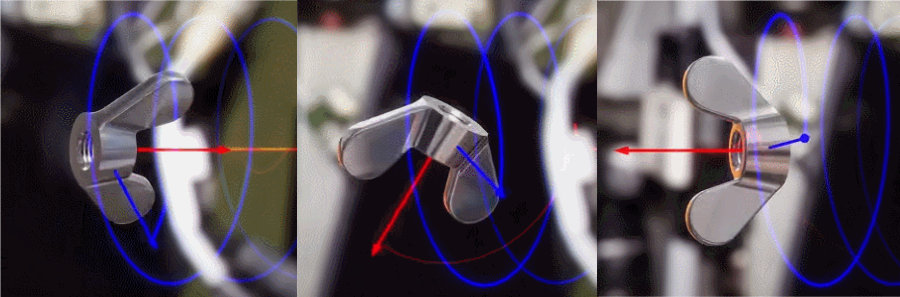
\includegraphics[width=0.9\textwidth]{dzhani.jpg}
\end{center}
   \caption{Ilustrasi efek Dzhanibekov \cite{28}.}
\label{fig:10}
\end{figure*}

Prinsip dasar di balik terjadinya perubahan mendadak pada sumbu rotasi Bumi terletak pada hukum fisika benda berputar. Contoh klasik yang menggambarkan fenomena ini adalah efek Dzhanibekov, yang pertama kali diamati oleh kosmonot Rusia, Vladimir Dzhanibekov \cite{37}, dan divisualisasikan dalam Gambar \ref{fig:10}. Dalam fisika, objek yang tidak berputar dengan sempurna pada salah satu dari tiga sumbu inersia utamanya tidak akan mempertahankan sumbu rotasi yang tetap. Jika objek tersebut berotasi dekat dengan sumbu utama kedua, maka objek tersebut akan mengalami perubahan arah rotasi yang tampak tiba-tiba. Meskipun ini tidak persis seperti yang kami yakini terjadi saat pembalikan Bumi, prinsip utamanya tetap berlaku: tanpa adanya gaya eksternal, perubahan mendadak sumbu rotasi hanya dapat dijelaskan melalui dinamika fisika rotasi.

Secara lebih spesifik, Bumi hampir pasti tidak mengalami efek Dzhanibekov yang sederhana dan seragam. Jika demikian, kita seharusnya bisa mengamati pergeseran bertahap pada sumbu rotasi Bumi dari waktu ke waktu. Namun, kami meyakini bahwa Bumi justru mengalami gangguan struktural yang bersifat periodik secara tiba-tiba, yang menyebabkan terjadinya pelepasan antara "lapisan rotasi luar" (kerak dan mantel) dan "badan rotasi dalam" (inti Bumi). Dalam sistem tertutup tanpa pengaruh luar, hukum kekekalan momentum sudut menyatakan bahwa Bumi tidak dapat mengubah arah sumbunya secara tiba-tiba. Oleh karena itu, pelepasan antara bagian dalam dan luar tubuh rotasi Bumi menjadi salah satu mekanisme internal yang dapat menjelaskan terjadinya pembalikan mendadak sumbu rotasi, selain dampak eksternal seperti tumbukan asteroid, yang dapat menyebabkan perubahan sumbu secara tiba-tiba.

Mekanisme spesifik yang diyakini memicu gangguan internal Bumi ini adalah perubahan wujud pada struktur besi yang membentuk inti Bumi (Gambar \ref{fig:11}). Inti dalam Bumi terutama terdiri dari besi (Fe) yang tersusun dalam struktur kristal heksagonal tumpukan-padat atau hexagonal close-packed (hcp) \cite{141}. Ketika struktur hcp-Fe ini mengalami perubahan wujud menjadi logam cair, sejumlah besar energi kinetik dilepaskan dan ditransfer ke inti luar. Proses perubahan wujud ini mengurangi permeabilitas magnetik inti, sehingga melemahkan medan geomagnetik dan melepaskan panas ke sekitarnya. Panas tersebut kemudian menciptakan struktur LLVP (Large Low-Velocity Shear Province/Daerah Besar dengan Pergeseran Berkecepatan Rendah) di mantel (Gambar \ref{fig:12}) \cite{38}, serta meningkatkan temperatur di permukaan Bumi, terutama melalui pemanasan laut dalam. Kedua fenomena ini telah didokumentasikan dengan baik dalam beberapa abad terakhir dan akan dibahas lebih lanjut dalam makalah ini.

\begin{figure*}[t]
\begin{center}
% \fbox{\rule{0pt}{2in} \rule{.9\linewidth}{0pt}}
\includegraphics[width=1\textwidth]{layers.jpg}
\end{center}
   \caption{Ilustrasi proses di dalam Bumi yang menyebabkan pembalikan ECDO \cite{129}.}
\label{fig:11}
\end{figure*}
\begin{figure}[t]
\begin{center}
% \fbox{\rule{0pt}{2in} \rule{0.9\linewidth}{0pt}}
   \includegraphics[width=1\linewidth]{llvp.jpg}
\end{center}
   \caption{Penggambaran detail LLVP di bawah Afrika Selatan \cite{28}.}
\label{fig:12}
\label{fig:onecol}
\end{figure}

Proses yang sama juga terjadi di dalam Bumi, namun dalam arah yang berlawanan. Hal ini diyakini mendorong perpindahan kembali ke keadaan rotasi Bumi saat ini dalam waktu yang relatif singkat setelah peristiwa pembalikan terjadi.

\section{Bukti Mengenai Pembalikan Bumi yang Akan Terjadi}

Ada alasan kuat untuk meyakini bahwa kita berada di ambang terjadinya pembalikan bumi berikutnya. Bencana besar semacam ini tidak terjadi selama beberapa milenium terakhir, yang kira-kira sesuai dengan frekuensi kemunculannya berdasarkan catatan sejarah dan data geologis. Bukti terkuat yang mendukung kemungkinan pembalikan dalam waktu dekat berasal dari data geomagnetik terbaru, yang menunjukkan bahwa medan geomagnetik Bumi telah melemah selama kurang lebih dua ribu tahun terakhir. Proses pelemahan ini terus meningkat dan dalam beberapa dekade terakhir telah mencapai tingkat yang mengkhawatirkan.

Terlihat pada Gambar \ref{fig:14} adalah medan geomagnetik Bumi pada tahun 1590 dan 2025 \cite{125,126}. Seperti yang diperlihatkan pada gambar, medan tersebut telah melemah secara signifikan.

Salah satu indikator lain dari melemahnya medan geomagnetik Bumi adalah pergerakan posisi kutub utara geomagnetik (Gambar \ref{fig:13}). Secara historis, kutub utara geomagnetik berada di wilayah Arktik Kanada. Namun, selama beberapa abad terakhir, posisinya perlahan-lahan bergeser, dan dalam beberapa dekade terakhir, pergeseran ini mengalami percepatan yang signifikan. Saat ini, kutub tersebut bergerak dengan cepat menuju Rusia, dengan kecepatan sekitar 55 kilometer per tahun \cite{124}.

\begin{figure*}[t]
\begin{center}
% \fbox{\rule{0pt}{2in} \rule{.9\linewidth}{0pt}}
\includegraphics[width=0.9\textwidth]{saa.jpg}
\end{center}
   \caption{Ilustrasi pelemahan medan geomagnetik dari tahun 1590 hingga 2025. Dihitung menggunakan model gufm1 dan IGRF-14 \cite{125,126}.}
\label{fig:14}
\end{figure*}

\begin{figure}[t]
\begin{center}
% \fbox{\rule{0pt}{2in} \rule{1\linewidth}{0pt}}
   \includegraphics[width=1\linewidth]{npw.jpg}
\end{center}
   \caption{Posisi kutub utara geomagnetik dari tahun 1590 hingga 2025, ditampilkan dalam interval 5 tahun \cite{142}.}
\label{fig:13}
\label{fig:onecol}
\end{figure}

\begin{figure}[t]
\begin{center}
% \fbox{\rule{0pt}{2in} \rule{1\linewidth}{0pt}}
   \includegraphics[width=1\linewidth]{ocean-highlight.jpg}
\end{center}
   \caption{Laju pemanasan laut dalam (kedalaman $>$2000 m) dari tahun 1991 hingga 2010, dilingkari merah \cite{132}.}
\label{fig:15}
\label{fig:onecol}
\end{figure}

Medan magnet Bumi diyakini dihasilkan oleh suatu dinamo internal—yakni aliran magma berbentuk kolom melingkar yang bergerak di dalam inti luar Bumi akibat rotasi planet ini \cite{123}. Melemahnya medan geomagnetik merupakan gejala dari gangguan yang terjadi jauh di dalam interior Bumi. Menurut teori ECDO, gangguan tersebut menyebabkan pelepasan panas dan pada akhirnya memicu terlepasnya keterkaitan antara mantel dan inti Bumi, yang kemudian mengakibatkan terjadinya pembalikan Bumi \cite{1}.

Terdapat banyak data yang mendukung keberadaan proses eksotermik di dalam interior Bumi. Pemanasan Bumi dicatat melalui peningkatan suhu permukaan benua dan lautan \cite{127,128}, serta peningkatan kadar CO$_2$ atmosfer yang bergerak seiring dengan kemunculan gumpalan panas dari dalam Bumi \cite{129,130}, dan juga melalui penurunan luas es laut global \cite{131}. Data-data ini menunjukkan bahwa peningkatan kadar CO$_2$ dan suhu bukanlah penyebab utama perubahan iklim yang disebut "buatan manusia", melainkan dampak lanjutan dari aktivitas eksotermik yang berasal dari inti Bumi \cite{129}.

Yang paling signifikan, studi mengenai laju pemanasan di laut dalam (kedalaman $>$2000 meter) menunjukkan bahwa tidak hanya lapisan dalam lautan yang mengalami pemanasan, tetapi tingkat pemanasan tertinggi justru ditemukan di lapisan abisal (4000–6000 meter). Pemanasan laut dalam ini memiliki titik pusat (centroid) di bawah kedalaman 4000 meter \cite{132,129}, yang secara fisik tidak mungkin terjadi jika pemanasan berasal dari atas, yakni atmosfer. Data ini memberikan dukungan kuat terhadap argumen bahwa perubahan iklim dan geomagnetik terbaru didorong oleh proses-proses yang terjadi jauh di dalam Bumi. Gambar \ref{fig:15} menunjukkan laju pemanasan laut dalam secara global dari tahun 1991 hingga 2010 \cite{132}.

\section{Pemodelan Pembalikan Bumi yang Akan Datang}
\begin{figure}[b]
\begin{center}
% \fbox{\rule{0pt}{2in} \rule{1\linewidth}{0pt}}
   \includegraphics[width=1\linewidth]{saa-crop.jpeg}
\end{center}
   \caption{Perhitungan titik kritis berdasarkan Anomali Atlantik Selatan menunjukkan perkiraan tanggal 13 Maret 2059 sebagai waktu terjadinya peristiwa tersebut. \cite{125,126}.}
\label{fig:16}
\label{fig:onecol}
\end{figure}

Memprediksi waktu terjadinya pembalikan Bumi berikutnya merupakan tugas yang kompleks. Saat ini, model terbaik yang tersedia untuk hal ini berasal dari medan geomagnetik Bumi—khususnya Anomali Atlantik Selatan (SAA). Wilayah ini, yang terletak di atas Samudra Atlantik bagian selatan, memiliki kekuatan medan geomagnetik paling lemah dan didefinisikan sebagai area dengan kekuatan medan di bawah 32.000 nanotesla \cite{135}, yang merupakan nilai terlemah yang tercatat pada tahun 1590. Luas permukaan Anomali Atlantik Selatan meningkat dari 1\% dari luas total permukaan Bumi pada tahun 1590 menjadi 21\% pada tahun 2025 \cite{136}.

Untuk memperkirakan kapan pembalikan Bumi dapat terjadi, saya melakukan pemodelan terhadap data perluasan permukaan Anomali Atlantik Selatan (SAA) menggunakan persamaan titik kritis dengan hukum pangkat. Persamaan ini digunakan untuk menggambarkan perilaku sistem kompleks yang sedang mendekati transisi kritis, yaitu suatu kondisi di mana sistem mengalami perubahan yang drastis dan tiba-tiba. Hasil perhitungan saya menghasilkan prediksi tanggal titik kritis pada 13 Maret 2059 (Gambar \ref{fig:16}). Akurasi prediksi ini akan semakin meningkat seiring dengan semakin dekatnya kita dengan masa transisi tersebut \cite{136}.

Metrik lain seperti pergeseran sumbu rotasi, anomali cuaca, serta data seismik dan vulkanik juga dapat membantu kita untuk mendapatkan prediksi yang lebih baik tentang kapan kemungkinan terjadinya pembalikan Bumi berikutnya.

\section{Linimasa Historis ECDO}

Meskipun menetapkan linimasa yang tepat untuk peristiwa ECDO di masa lalu merupakan hal yang sulit, tampaknya setidaknya telah terjadi dua peristiwa ECDO selama periode Holosen. Catatan dari Herodotus, yang ia peroleh dari para imam Mesir, menyebutkan bahwa \textit{"sejak raja pertama hingga pendeta Hephaistos terakhir, telah ada tiga ratus empat puluh satu generasi manusia... Dalam kurun waktu tersebut, mereka mengatakan bahwa matahari telah empat kali berpindah dari tempat terbit biasanya; tempat ia sekarang terbenam dulunya adalah tempat ia dua kali terbit, dan tempat ia sekarang terbit adalah tempat ia dua kali terbenam"} \cite{32}. Plato, yang hidup pada abad ke-5 SM \cite{111}, juga menyatakan bahwa setelah banjir besar yang menenggelamkan Atlantis dalam satu hari dan satu malam, sekitar 9.000 tahun sebelumnya, \textit{"telah terjadi banyak banjir sejak saat itu, dan orang-orang yang selamat di pegunungan kehilangan pengetahuan tentang tulis-menulis, dan selama banyak generasi hanya berfokus pada upaya bertahan hidup"} \cite{112}. Pernyataan ini mengindikasikan bahwa kemungkinan telah terjadi lebih dari dua kali pembalikan sejak berakhirnya periode Younger Dryas sekitar tahun 9700 SM. Bukti fisik yang dibahas dalam makalah ini serta dalam penelitian saya sebelumnya \cite{2} memberikan dukungan kuat terhadap catatan yang disampaikan oleh Plato.

Perkiraan waktu terakhir kali terjadinya pembalikan ECDO diperkirakan terjadi antara tahun 2300 hingga 1600 SM, suatu periode yang dikaitkan dengan berbagai catatan bencana banjir besar (seperti kisah Gun-Yu \cite{113,114,115}, Ogyges \cite{116,117}, Peru \cite{118,119}, dan Kitab Keluaran \cite{120}), kehancuran dan pengabaian peradaban (seperti Mohenjo-Daro \cite{121} dan Kreta Minoa \cite{100,101}), serta anomali fisik (seperti peristiwa Bond \cite{122} dan peristiwa 4.2 ribu tahun \cite{90}). Hingga saat ini, belum ditemukan konvergensi bukti yang cukup kuat setelah periode tersebut yang menunjukkan terjadinya peristiwa katastropik besar berskala global.

\section{Kesimpulan}

Operasi NANOOK adalah upaya pengintaian pada era Perang Dingin yang dilakukan oleh Amerika Serikat untuk memetakan wilayah Arktik dan pesisir utara Uni Soviet setelah Perang Dunia II \cite{137}. Dalam proses penyelidikannya, mereka menemukan bahwa kutub magnetik berada 125 hingga 200 mil ke arah utara dari posisi yang diperkirakan berdasarkan ekspedisi-ekspedisi sebelumnya. Sehubungan dengan temuan ini, \textit{"Di kalangan ilmuwan pemerintah, muncul pertanyaan mengenai apa yang akan terjadi jika kutub magnetik dan kutub geografis saling berimpit. Untuk menjawabnya, di bawah kendali proyek oleh Dr. Paul A. Siple, Rand Corporation dikontrak untuk melakukan studi laboratorium menggunakan model bumi yang terdiri dari dua bola konsentris—bola dalam mewakili inti besi cair bermuatan elektromagnetik yang porosnya menentukan posisi kutub "magnetik", dan bola luar mewakili kerak bumi yang berputar di sekitar poros kutub "geografis". Melalui eksperimen berulang, ditemukan bahwa saat kutub "magnetik" mendekati kutub "geografis", pada titik tertentu kutub magnetik akan mempercepat laju konvergensinya seolah-olah tertarik oleh gaya sentripetal menuju kutub "geografis" dan kemudian meloncat untuk berimpit dengannya; namun, alih-alih berimpit, kutub "magnetik" justru akan secara tiba-tiba "membalik" mengelilingi kutub "geografis", lalu terlempar menuju ekuator seolah-olah terdorong oleh gaya sentrifugal, dan akhirnya berhenti pada posisi di mana kedua poros membentuk sudut divergensi sekitar 89 derajat. Setelah peristiwa "pembalikan" kutub ini terjadi, kedua poros kemudian secara bertahap mulai mendekat kembali dalam rentang waktu yang lama"} \cite{138,139}.

Selanjutnya, \textit{"Dalam salah satu pertemuan ilmiah yang dihadiri Mayor White di Pentagon pada awal tahun 1948, para ilmuwan membahas apakah sebaiknya masyarakat diberi tahu mengenai fenomena pembalikan kutub yang akan datang. Tidak ada satu pun ilmuwan yang setuju untuk menyembunyikan informasi ini dari publik; namun di sisi lain, mereka juga tidak sepakat mengenai cara terbaik untuk mengumumkannya. Beberapa dari mereka khawatir bahwa pengetahuan tentang fenomena ini dapat merusak tatanan moral masyarakat. Namun kekhawatiran tersebut tampaknya tidak terbukti, karena pada awal 1950-an informasi tentang fenomena pembalikan kutub telah dipublikasikan baik dalam kolom surat kabar dan artikel majalah—namun secara mengejutkan tidak menimbulkan tanggapan apa pun dari publik yang sepertinya terkejut, berpikiran sempit, atau tidak percaya"} \cite{138,139}.

Mengapa kita tidak memperhatikan hal ini? Terdapat banyak alasan kuat untuk meyakini bahwa Bumi pernah mengalami pembalikan sebelumnya. Makalah ini, beserta bagian keduanya, menyajikan ringkasan padat dari berbagai bukti yang saling menguatkan dari banyak bidang yang menunjukkan bahwa peristiwa tersebut memang pernah terjadi. Bukti-bukti tersebut mencakup kisah banjir besar dari berbagai budaya di seluruh dunia, keberadaan fosil laut dan endapan garam di daratan, tempat perlindungan bawah tanah kuno, sisa-sisa hewan, serta bentang alam geologi yang menunjukkan tanda-tanda bencana besar. Manusia diperkirakan telah ada selama ratusan ribu tahun, namun catatan sejarah modern hanya mencakup beberapa ribu tahun terakhir. Mungkinkah ini menunjukkan bahwa dari waktu ke waktu, Bumi mengalami pembalikan kutub, benua-benua tersapu bersih, dan umat manusia dipaksa untuk memulai kembali dari awal—kembali ke Zaman Batu—hingga catatan sejarah purba yang tersisa hanyalah kisah-kisah bencana besar? Jika demikian, maka mencegah terulangnya peristiwa ini mungkin merupakan salah satu tugas terpenting umat manusia.

Sebagai penutup, saya ingin menyampaikan sebuah kisah yang tercatat dalam Timaeus karya Plato, yang menggambarkan percakapan antara Solon, seorang negarawan Athena, dengan para pendeta Mesir \cite{140}: \textit{“Pada suatu kesempatan, ketika Solon berusaha mengajak para pendeta berdiskusi tentang sejarah kuno, ia mulai menceritakan tradisi paling tua dari bangsanya, termasuk kisah Phoroneus—yang dikatakan sebagai manusia pertama—dan Niobe. Ia juga menceritakan legenda tentang Deucalion dan Pyrrha setelah peristiwa Banjir Besar, serta bagaimana mereka selamat dan menurunkan generasi berikutnya. Ia bahkan mencoba menghitung rentang waktu kejadian tersebut berdasarkan silsilah keturunan mereka. Mendengar hal itu, salah satu pendeta yang sangat tua berkata, "Wahai Solon, Solon, kalian orang Yunani selalu seperti anak-anak; tidak ada yang benar-benar tua di antara kalian." Ketika Solon bertanya apa maksud dari ucapan itu, pendeta menjawab, "Jiwa kalian semua masih muda. Kalian tidak memiliki satu pun kepercayaan yang berasal dari tradisi kuno, ataupun satu pun ilmu pengetahuan yang tak lekang oleh waktu. Sebabnya adalah karena telah terjadi dan akan terus terjadi banyak kehancuran umat manusia, baik yang besar akibat api dan air, maupun yang kecil melalui berbagai cara lainnya. Kisah yang kalian ceritakan di negeri kalian maupun di sini tentang Phaethon, putra Helios, yang mencoba mengendarai kereta matahari ayahnya namun gagal mengendalikannya hingga membakar bumi dan akhirnya dihantam petir—itu hanya tampak seperti mitos. Namun sebenarnya, kisah itu menggambarkan pergeseran benda-benda langit yang mengelilingi bumi dan kehancuran di bumi akibat api hebat yang terjadi berulang kali dengan selang waktu yang lama. Pada masa-masa seperti itu, mereka yang tinggal di pegunungan atau dataran tinggi lebih menderita dibandingkan mereka yang tinggal di dekat sungai atau laut. Di negeri kami, Sungai Nil menjadi penyelamat kami, tidak hanya dalam kehidupan sehari-hari, tetapi juga saat terjadi bencana besar seperti ini, karena ia naik dan membanjiri wilayah kami. Sebaliknya, ketika para dewa menyucikan bumi dengan banjir besar, para penggembala yang tinggal di pegunungan selamat, sedangkan mereka yang tinggal di kota-kota seperti milikmu tersapu arus dan hanyut ke laut. Di negeri kami, air tidak pernah datang melalui hujan dari atas dan mengguyur ladang, melainkan selalu muncul dari bawah permukaan tanah. Karena alasan-alasan inilah, pengetahuan kuno lebih terjaga di sini; dan pada dasarnya, di tempat mana pun yang tidak terlalu panas atau terlalu dingin, umat manusia akan selalu bertahan—meskipun kadang dalam jumlah kecil. Setiap kejadian besar atau penting yang pernah terjadi—baik di negerimu, di negeri kami, maupun di tempat-tempat lain yang kami ketahui melalui laporan—semuanya dicatat sejak dahulu kala dan disimpan di kuil-kuil kami. Sementara itu, bangsa kalian dan bangsa lain selalu kembali menjadi seperti baru, seiring dengan hancurnya catatan dan pengetahuan akibat siklus kehancuran, dengan banjir besar seperti wabah dari langit yang datang kembali setiap beberapa ribu tahun. Ketika itu terjadi, hanya yang tidak bisa membaca atau menulis yang selamat, dan seluruh peradaban harus mulai dari awal tanpa ingatan terhadap masa lalu. Silsilah yang kau sebutkan tadi, Solon, tentang rakyatmu, nyaris seperti cerita anak-anak. Kalian hanya mengingat satu peristiwa banjir, padahal banyak yang telah terjadi sebelumnya. Kalian juga tidak mengetahui bahwa bangsa yang paling luhur dan sempurna pernah hidup di wilayah yang kini kalian tempati. Dari mereka pula dirimu dan seluruh kotamu berasal, dari benih kecil yang berhasil selamat. Namun kalian tidak mengetahuinya karena mereka yang selamat pada masa itu tidak mampu menuliskannya. Sesungguhnya, Solon, sebelum kehancuran terbesar akibat air, negara yang sekarang merupakan Athena dulunya adalah kekuatan militer yang paling unggul dan sangat terorganisir dalam segala aspek. Konon, mereka memiliki karya seni yang agung dan pemerintahan yang paling mulia dari semua bangsa yang pernah kami dengar.”}

Para pendeta yang sama juga menceritakan kepada Solon tentang peradaban kuno Atlantis: \textit{“Segala sesuatu yang ada di wilayah kami ini, yang berada di balik mulut yang kami maksud, tampak jelas adalah sebuah pelabuhan dengan pintu masuk yang sempit. Namun wilayah di seberangnya adalah lautan sejati, dan daratan yang mengelilinginya lebih layak disebut sebagai sebuah benua, dalam arti yang sepenuhnya. Di pulau Atlantis tersebut dahulu terdapat sebuah konfederasi raja-raja yang memiliki kekuasaan besar dan luar biasa, yang menguasai seluruh pulau itu, banyak pulau lainnya, serta sebagian wilayah benua. Mereka bahkan menguasai daerah-daerah di dalam Selat Herakles, yaitu Libya hingga Mesir, dan Eropa hingga wilayah Tyrrhenia. Kekuatan gabungan mereka pernah, dalam satu serangan besar, berupaya menaklukkan dan memperbudak wilayahmu, wilayah kami, dan seluruh daerah yang berada di dalam batas selat tersebut. Namun pada saat itulah, wahai Solon, bangsa Athenamu menunjukkan keberanian dan kekuatan yang luar biasa di mata dunia. Mereka unggul dalam keberanian dan keahlian militer, dan dengan bertindak sebagai pemimpin sebagian bangsa Yunani, atau bahkan berjuang sendirian ketika ditinggalkan oleh sekutu-sekutunya, mereka menghadapi bahaya yang paling mematikan, mengalahkan para penyerbu, dan mendirikan monumen kemenangan. Melalui kemenangan itu, mereka menyelamatkan bangsa-bangsa dari perbudakan, dan dengan kemurahan hati membebaskan seluruh penduduk di wilayah dalam batas-batas Herakles. Namun, pada masa berikutnya, terjadi gempa bumi dan banjir besar yang luar biasa. Dalam satu hari dan malam yang mengerikan, seluruh pasukan tangguh dari negaramu ditelan oleh bumi, dan pulau Atlantis pun mengalami nasib yang sama—tenggelam ke dalam laut dan lenyap.”}

\section{Ucapan Terima Kasih}

Terima kasih kepada Ethical Skeptic, penulis asli tesis ECDO, atas selesainya tesis yang penuh wawasan dan terobosan serta telah membagikannya kepada dunia. Tesis trilogi beliau \cite{1} tetap menjadi karya penting bagi teori Osilasi Dzhanibekov Pelepasan Inti-Mantel Eksotermik (ECDO: Exothermic Core-Mantle Decoupling Dzhanibekov Oscillation), dan memuat jauh lebih banyak informasi tentang topik ini daripada yang telah saya bahas secara singkat di sini.

Terima kasih kepada Ankit, yang telah memproses data kompilasi bencana pada Tabel 1.

Dan tentu saja, terima kasih kepada orang-orang besar yang telah berjasa; orang-orang yang telah melakukan semua penelitian dan penyelidikan yang memungkinkan karya ini dapat ditulis dan telah berupaya membawa pencerahan bagi umat manusia.

\clearpage
\twocolumn

\section{Gambar-gambar Tambahan}


\begin{figure}[H]
\begin{center}
% \fbox{\rule{0pt}{2in} \rule{1\linewidth}{0pt}}
   \includegraphics[width=1\linewidth]{wave.jpg}
\end{center}
   \caption{Sebuah pengamatan mendalam terhadap pola erosi gelombang berbentuk parabola yang mengikis bagian bawah Piramida Khafre\cite{27}.}
\label{fig:19}
\label{fig:onecol}
\end{figure}

\begin{figure}[H]
\begin{center}
% \fbox{\rule{0pt}{2in} \rule{1\linewidth}{0pt}}
   \includegraphics[width=1\linewidth]{star-stone.jpg}
\end{center}
   \caption{Peta bintang yang dipahat pada batu di salah satu poros piramida Khufu \cite{28}.}
\label{fig:20}
\label{fig:onecol}
\end{figure}

\begin{figure*}[t]
\begin{center}
% \fbox{\rule{0pt}{2in} \rule{.9\linewidth}{0pt}}
\includegraphics[width=1\textwidth]{deepsea.jpg}
\end{center}
   \caption{Gambar anomali pemanasan laut dalam dan abisal dibandingkan dengan kurva pemanasan laut atmosfer normal. Anomali pemanasan secara keseluruhan diambil dari NOAA \cite{147}, distribusi pemanasan dalam dan abisal dari studi Desbruyeres \cite{132}, serta pemrosesan data dan visualisasi oleh Ethical Skeptic \cite{129}.}
\label{fig:21}
\end{figure*}

\begin{figure*}[t]
\begin{center}
% \fbox{\rule{0pt}{2in} \rule{.9\linewidth}{0pt}}
\includegraphics[width=1\textwidth]{sealevel.jpeg}
\end{center}
   \caption{Permukaan laut menunjukkan peningkatan variansi sebesar 20\% selama 75 tahun di 63 stasiun, mengindikasikan peningkatan kecepatan arus. Lonjakan variansi permukaan laut terjadi bersamaan dengan gelombang panas lautan, menunjukkan bahwa keduanya mungkin disebabkan oleh pemanasan dari dalam laut Bumi \cite{2,129}.}
\label{fig:22}
\end{figure*}

\begin{figure*}[t]
\begin{center}
% \fbox{\rule{0pt}{2in} \rule{.9\linewidth}{0pt}}
\includegraphics[width=1\textwidth]{co2.jpg}
\end{center}
   \caption{Kadar CO2 di dalam atmosfer telah meningkat secara konsisten selama 45 tahun terakhir, kemungkinan disebabkan oleh kenaikan suhu laut. Sumber: NOAA \cite{148,129}.}
\label{fig:23}
\end{figure*}

\begin{figure*}[t]
\begin{center}
% \fbox{\rule{0pt}{2in} \rule{.9\linewidth}{0pt}}
\includegraphics[width=1\textwidth]{ice.jpg}
\end{center}

   \caption{Luas es laut global telah menyusut selama 45 tahun terakhir, akibat Bumi yang memanas. Sumber: ADS \cite{149}.}
\label{fig:24}
\end{figure*}

\clearpage
\twocolumn

{\small
\renewcommand{\refname}{Referensi}
\bibliographystyle{ieee}
\bibliography{egbib}
}

\end{document}